\section{DroneCharge}
\subsection{Vision}
DroneCharge was envisioned as a framework to be used by drone application developers to easily achieve task-execution using swarms of drones, and as such needed to fit any and all suitable drones. As all drones have their own native APIs for control, this meant that a driver-oriented architecture had to be utilized. While the drivers provided us with means of controlling the drone, we also needed a way of hooking into the tasks performed by the drones in order to seamlessly exchange drones when rquired. This was done by having developers define tasks in terms of a series of subtasks, and to have our framework execute those tasks in the right order. That enabled us to hook into the execution of a task and to exchange drones when a recharge was needed.

\subsection{Architecture}
Our overall architecture is depicted in Figure \ref{fig:architecturefig}. The most interesting concepts are the ideas of drone, task and environment. A task is performed in an environment that has a number of drones at its disposal, all of which are configured by the individual developer. As a developer, you would implement drivers for your specific drone that inherits from the drone class, and either utilize the built-in tasks or create your own extending from the task class. A drone instance representing each physical drone is then added to the environment along with their respective charging locations, as well as any number of tasks to be performed.

\begin{figure}[h]
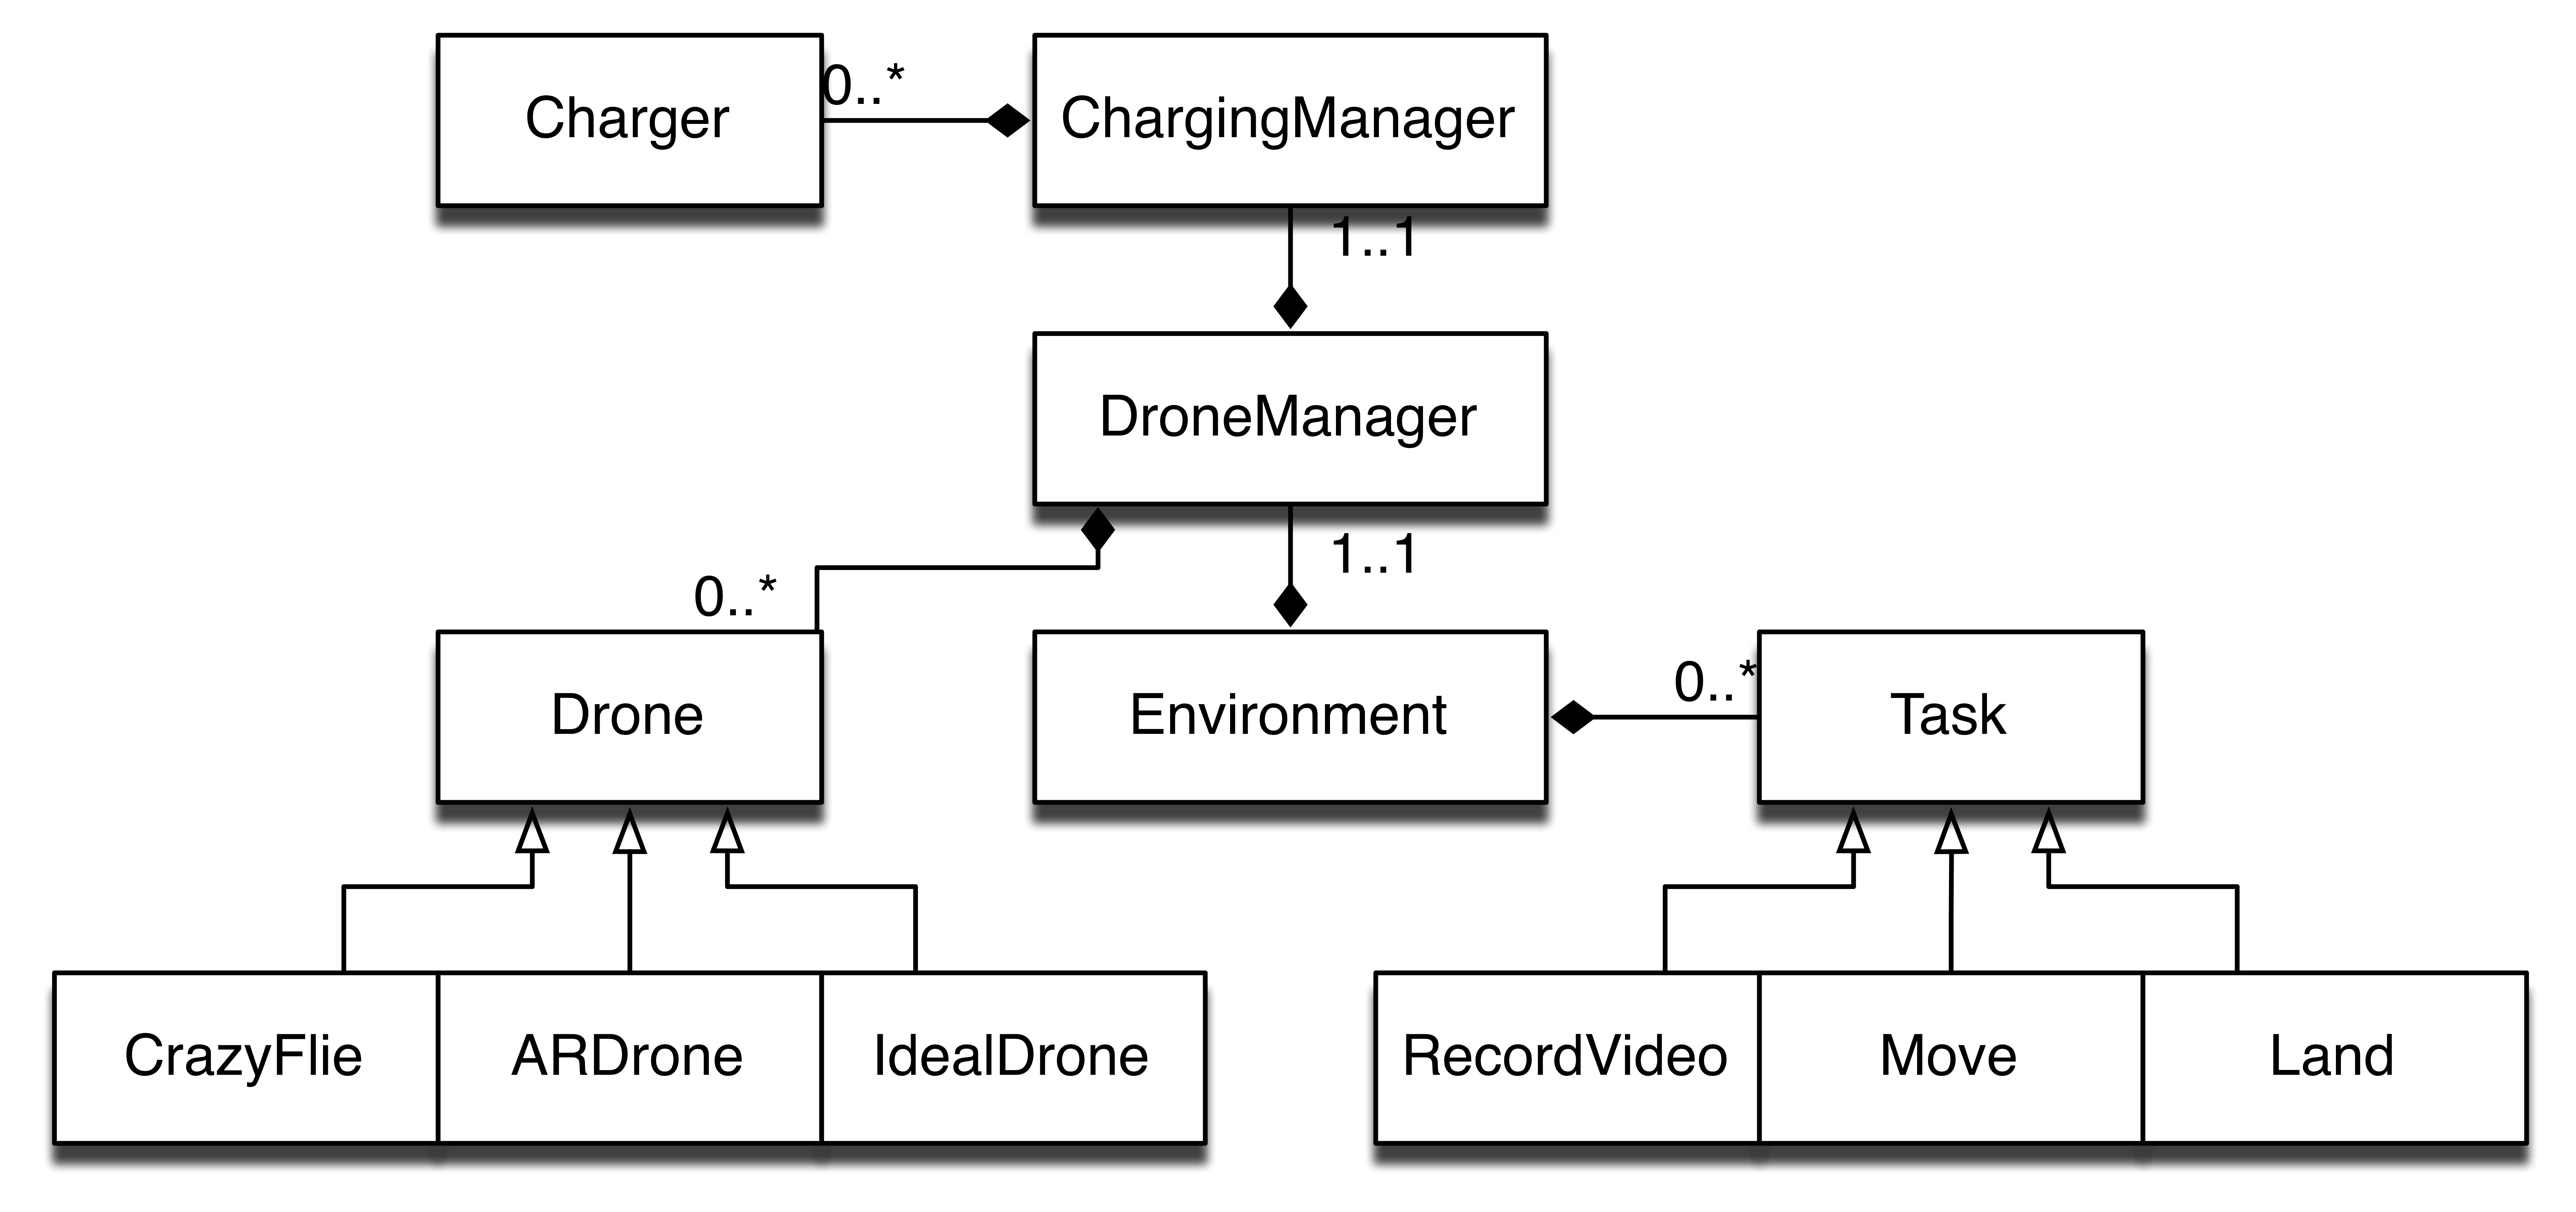
\includegraphics[width=0.5\textwidth]{images/dronechargearchitecture.png}
\caption{DroneCharge architecture}
\label{fig:architecturefig}
\end{figure}

\subsection{Drivers}
Drivers are, as is the definition, a way for the system to interact with the hardware devices connected to it without knowing the hardware specifications at compile-time. In our case, those hardware devices are drones and their locationing system. Any developer using DroneCharge must implement a class extending from the Drone-class that implements neccesary features such as movement as well as battery- and location-queries. These are called drone-drivers. Whether a drone has positioning built-in or if it uses a tertiary system such as tracking with a Microso Kinect is irrelevant, as long as the drone-driver has the ability to obtainin its position.

\subsection{Tasks}
Tasks define how individual steps of a task are performed. They contain a list of capabilities required to perform the task such as movement or video-recording, as well as instructions on how to perform the task. DroneCharge comes with a limited number of built-in tasks such as movement and landing, but any task can be performed by extending the task class and explicitly performing the task through the commands defined in the drone-drivers. The framework will only assign drones to perform the task if they meet the requirements for it, so you are guaranteed to have the right type of drone as long as your task and required capabilities are aligned. As an example, a custom driver for a drone with a video camera attached to it could implement a function called \textit{RecordVideo} as well as contain the capability \textit{recordvideo}. You could then define a task whose execution consisted of turning on a video camera. By specifying \textit{recordvideo} as a required capability of the task, the framework would not perform the task until a drone with said capability was available.
\subsubsection{The Task Tree}
By allowing tasks to be added to other tasks, we obtained a tree-structure view of tasks which enabled us to do a depth-first search traversel of tasks, and in that way achieve a sound logical structuring of tasks and subtasks. The tree is traversed in such a way that only leaf-node-tasks are actually performed. This enabled developers to logically split their tasks into subtrees however they saw fit and gave us increased flexibility.

\subsection{Assumptions and requirements}
When using the DroneCharge framework, developers must be aware of the assumptions and requirements made in terms of the capabilities and implementation of the drivers.

For the drone drivers, we assume that a drone or its driver can report its battery level in a linear fashion. That is, the battery cannot be reported as full untill the battery is depleted as is the case with some drones such as the CrazyFlie. Furthermore, there must be some way to obtain the position of the drone in relative or absolute terms. A developer must also define at what battery level the drone is to be considered low on battery.

In terms of defining tasks, we make the requirement that any single (sub)task must not require more battery to perform than is considered to be the low battery limit. That is, if the drone is considered to be at low battery when it reaches 10\%, all individual subtasks must require no more than 10\% power to perform. Finally, the point of operation that is the farthest from the charging station must not require a movement task using more battery power than is defined as being the low battery level to move to.

Additionally, it should be noted that a drone partaking in the execution of a task must have all capabilities  needed to perform all subtasks in the task tree in which the current subtask is located. This is upheld by the framework itself, as it will not choose drones lacking any capabilities.